%%%%%%%%%%%%%%%%%%%%%%%%%%%%%%%%%%%%%%%%%%%%%%%%%%%%%%%%%%%%%%%%%%%%%%%%%%%%%%%%
%%%%%%%%%%%%%%%%%%%%%%%%%%%%%%%%%%%%%%%%%%%%%%%%%%%%%%%%%%%%%%%%%%%%%%%%%%%%%%%%
%% Chapter - Related Work
%%%%%%%%%%%%%%%%%%%%%%%%%%%%%%%%%%%%%%%%%%%%%%%%%%%%%%%%%%%%%%%%%%%%%%%%%%%%%%%%
%%%%%%%%%%%%%%%%%%%%%%%%%%%%%%%%%%%%%%%%%%%%%%%%%%%%%%%%%%%%%%%%%%%%%%%%%%%%%%%%

\startchapter{Related Work}
\label{chap:relatedWork}

This thesis explores different approaches to allow scientists to view,
annotate and analyze large bioacoustic databases.  The study of
bioacoustics has a long and rich history, and in the first section of
this chapter, a brief summary of the history of bioacoustics in
general is presented.  Previous work done in analyzing the
vocalizations of \textit{Orcinus orca} is also reviewed.

In the following section, an overview of the literature on the use of
audio feature extraction to generate features suitable both for the
visualization of bioacoustic data and for use with machine learning
algorithms is presented.  A brief history of waveform-based
methods for visualization of sounds is provided, and this is
followed by reviews of the use of spectral based methods, including
sonograms, spectrograms and measures derived from spectrograms,
including Mel-Frequency Cepstral Coefficients and other descriptions
of spectra.  A brief overview of the field of pitch detection and of
the use of these methods in the study of bioacoustics is
provided.  Many of these pitch detection algorithms are complementary
to spectral based methods in that they often use autocorrelation
algorithms which detect correlations in a signal using a time based
representation of sound.

In order to allow scientists to listen to, view and perform analysis
on these large collections of audio, the use of computer-based tools
is a necessity.  In the past, researchers in bioacoustics would
analyze their data with programs on a single computer such as Raven
and MATLAB typically one file at a time.  I provide only a brief
search of the vast literature on the use of computer based tools to
view, annotate and analyze audio.  In ideal situations, these tools
provide for Intelligence Augmentation (IA)
\cite{biocca1996intelligence}, in which computer based tools do not
replace human intelligence but instead augment or improve it.  This
stands in contrast to the concept of Artificial Intelligence, where
tools that produce information independently of humans are used, with
the ultimate end of replacing the need for human intelligence.  IA
instead acknowledges that computers and humans have different
cognitive strengths and that for certain complex tasks an optimal
system would combine the best aspects of human and computer
intelligence.  This thesis examines the literature for evidence of
tasks that benefited from the use of IA and draws parallels between
these systems and the system described in this thesis that allows
scientists to view, annotate and analyze large bioacoustic databases.

Some of the largest hurdles in the study of large bioacoustic
databases is their vast size, the small number of researchers studying
these databases, and the messy nature of these databases.  In order to
assist scientists with large datasets, the use of citizen science and
crowdsourcing has been used for many years, with approaches as diverse
as the collection of word use for the Oxford English
Dictionary\cite{brody1999professor} \cite{goodchild2007world}, the use
of far-flung citizen scientists to aid Linnaeus with the study of
taxonomy\cite{linnaeus1758systema}, to the work of Dr. Fred Urquhart
in the study of monarch butterfly migrations\cite{howard2009fall}
\cite{oberhauser2008citizen}.  In recent years, the use of the
internet has enabled many more ways for interested members of the
public to help scientists study difficult problems, and I provide a
brief summary of the literature on this topic.  In this thesis, we
present a simple matching game to allow citizen scientists to assist
us in the classification of audio in a paradigm I call Serious Casual
Games.  I examine the literature on the use of gamification on the
study of complex phenomena and which aspects of gamification have shown
the most promise in previous studies.



\section{Bioacoustics}
\label{section:relatedWork:bioacoustics}

Humans have used sound to identify animals since prehistoric times;
some of the earliest extant literature comes from Aristotle.  In ``On
the Soul'' \cite{aristotle1}, he describes how animals make sound and
notes that while some sounds are produced by the ``impact of the
inbreathed air against the windpipe'' there are many other mechanisms
by which animals produce sound.  In ``The History of Animals''
\cite{aristotle2}, he describes a wide variety of sounds made by
animals from the ``low hiss'' of the tortoise, the ``peculiar croak''
of the frog, to the ``squeak and moans'' of a dolphin.

Animals make a wide variety of sounds, and humans have been interested
in and studied these sounds since the time of Aristotle and before.
The sounds made by animals are produced for a wide variety of purposes
from the echolocation clicks of bats, to alerting others to the
presence of threats, to communication for finding mates, and for other
kinds social interaction.  These sounds are often quite characteristic
of the species in question, and humans have long been able to identify
different animals by the sounds that they make.

The sounds produced by animals can be produced in a wide variety of
ways and can be of a wide range of frequencies and amplitudes.  The
range of human hearing is approximately 20 Hz to 20,000 Hz,
\cite{lyon1990cochlear} and while many animals make sound in this
range, others, such as bats, make sound in the ultrasonic range, while
others like elephants, produce sound below the range of human hearing.
The amplitude of sounds produced by animals is similarly diverse, with
some producing sounds inaudible to humans, while others like the blue
whale can produce sounds in excess of 188 decibels under water
\cite{clark2006acoustic}.

Before the advent of electro-mechanical and electronic recording
devices, sounds were often described by researchers using
transliterations of animal sounds onto human speech.  A simple example
is the song of the chickadee (\textit{Poecile} spp.), which is
represented in human speech with the words ``chick-a-dee-dee'', or the
sound of the tawny owl \textit{(Strix aluco)}, which is represented by
the words ``tu-whit tu-whoo''.  An interesting historical aside is
that in different languages, different words are used to represent the
sounds of animals, such as the ``meow'' of a cat in English, ``miaou''
in French, ``miyav'' in Turkish and ``nyan nyan'' in Japanese
\cite{weiss2011animals}.  Another interesting example is the different
representations of the sounds of roosters, which include ``Kukeleku''
in Dutch, ``Cocorico'' in French, ``Kickeriki'' in Italian,
``Quiquiriqui'' in the Basque language.

The earliest quantitative study of animal sounds began with the
recording of sounds onto wax cylinders, and the visualization of
sounds was a byproduct of the way that sound was recorded onto these
cylinders.  A photograph of a wax cylinder can be seen in Figure
\ref{fig:waxCylinder} with a series of test tones enscribed on it.  It
is clear to see the different patterns that the different sounds give.

\begin{figure}[t]
\centering
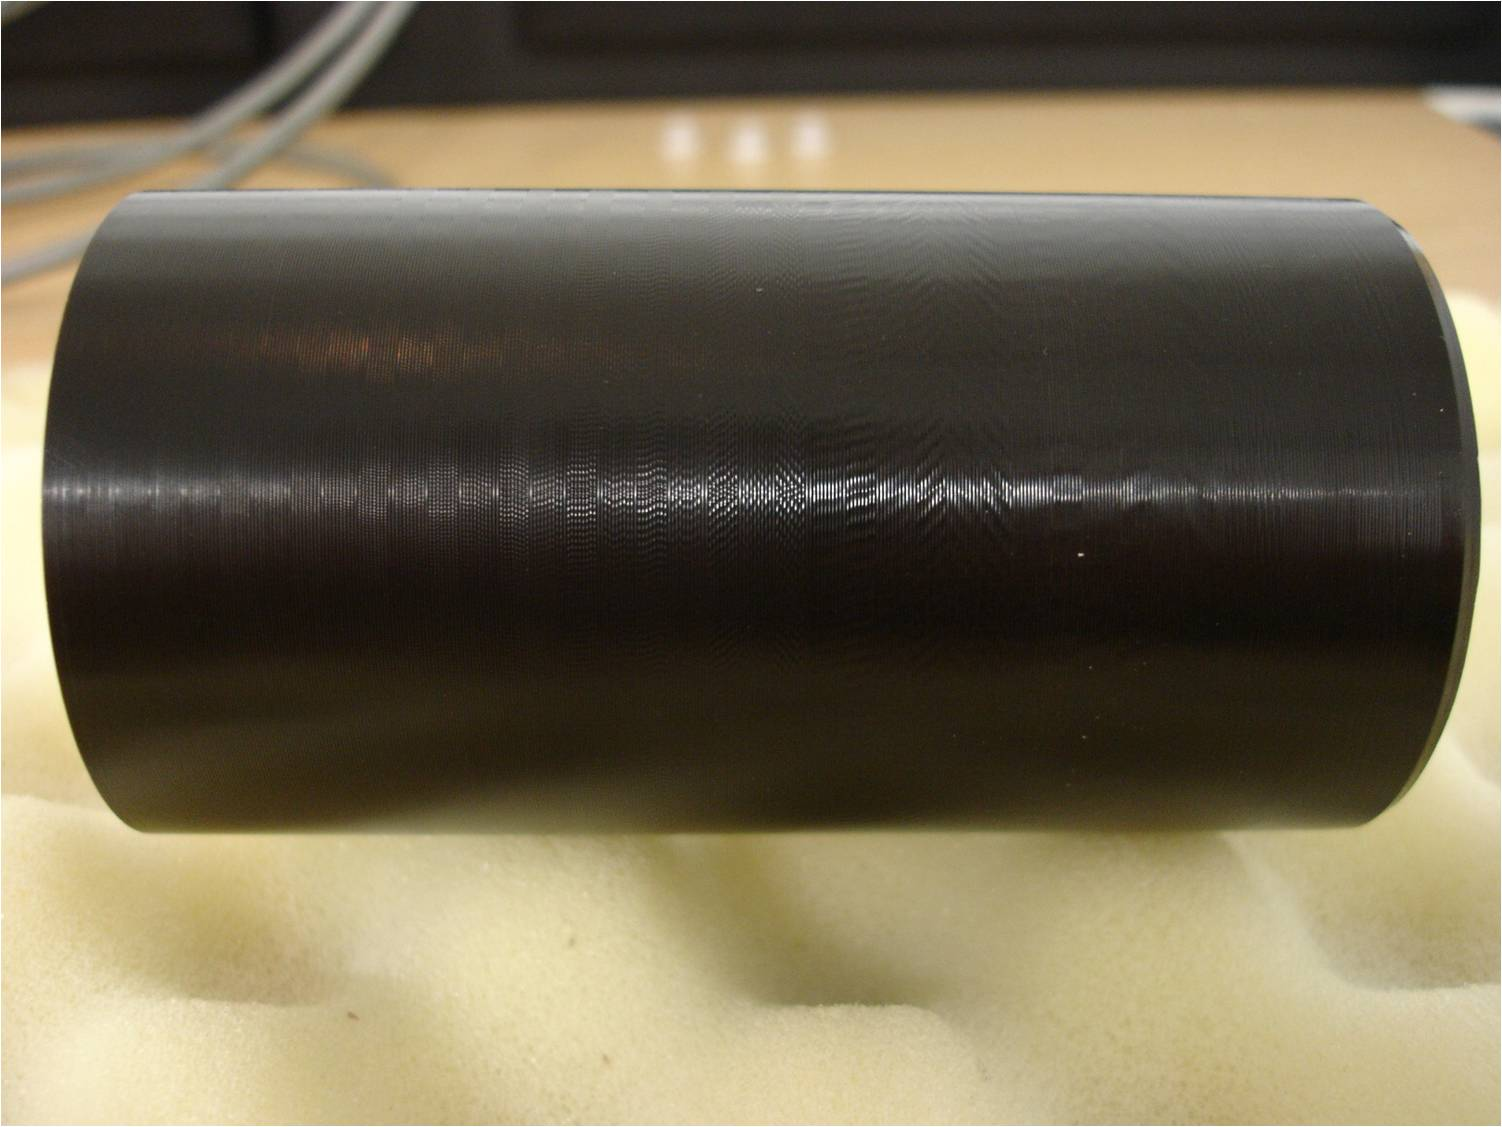
\includegraphics[width=\columnwidth]{figures/waxCylinder}
\caption{A wax cylinder with a series of test tones recorded onto it.
  Note the different patterns for the different frequencies of the
  test tones.}
\label{fig:waxCylinder}
\end{figure}


The creation of permanent recordings of animal sounds was a huge leap
forward for the field of bioacoustics as it allowed researchers to
record the sounds of animals and to listen to and analyze them in more
detail in a laboratory environment.  It also allowed the scientists to
distribute their recordings to other researchers and facilitated
scientific discourse in this field.

Early devices such as the Phonoautograph of Edouard-Lyon Scott de
Martinville developed in 1857 and the Phonodiek of Dayton C. Miller
developed in 1909 allowed for the visualization of the waveforms of
sounds, and Alexander Graham Bell created a device that permanently
recorded traces of sounds onto smoked-glass.  It is relatively
difficult to analyze bioacoustic sounds purely by their waveforms as
they are often composed of multiple overlapping harmonics, and the
relative phase of these harmonics can make sounds that sound similar
to the ear but look quite different when visualized as a waveform
\cite{au2000hearing}.

Bioacoustics is a scientific field of study that combines the fields
of biology and acoustics.  Although humans have used the sounds of
animals to identify and track them for many years, one of the first
researchers in this field was Ivan Regen who in 1925 systematically
studied the sounds of insects \cite{zarnik1929zivot}.  In the later
half of the 20th century, advances in electronic means of recording
and producing sound dramatically increased the breadth and scope of
the field of bioacoustics.  In recent years, the application of the
computational tools used in Music Information Retrieval have further
extended the possibilities of analyzing sound from biological sources.

Because of the sensitivity of humans and other animals to the
frequencies of sounds, devices that could separate sounds into their
characteristic frequency bands proved very useful in the study of
bioacoustics sounds.  The first such commercially available device was
the Sona-Graph, produced by the Kay Electric company.  A photograph of
this device can be seen in Figure \ref{fig:kayElectricSonagram}.

\begin{figure}[t]
\centering
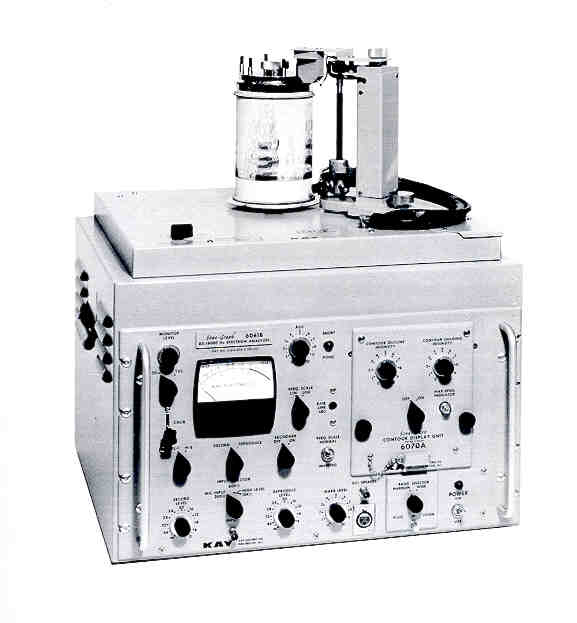
\includegraphics[width=90mm]{figures/kayElectricSonagram}
\caption{A photograph of the Kay Electric Company Sona-Graph.  This
  device was used by many researchers in bioacoustics before desktop
  computers became powerful enough to do the FFT calculation needed to
  make a spectrogram.  In this device, a heated needle would rotate
  around a cylinder.  The needle is tuned to a specific resonant
  frequency that varies over the course of drawing the spectrogram.
  If the needle resonated, it would touch the paper and burn it,
  showing the frequency, but giving off voluminous clouds of smoke in
  the process.  A typical 2 second orca vocalization would take the
  machine about 7 minutes to process \cite{lindblom1962accuracy}. }
\label{fig:kayElectricSonagram}
\end{figure}


This device produced a two-dimensional representation of sound, with
frequency along one axis and time along the other.  It had two
settings for the production of images, a narrow-band mode and a
wide-band mode.  The narrow-band mode had good frequency resolution at
the expense of time resolution; an example of this is shown in Figure
\ref{fig:sonagraph1}.  This setting had a frequency bandwidth of 45Hz
\cite{nowicki1988birds}.  The wide band mode emphasized time
resolution at the expense of frequency resolution with a frequency
bandwidth of 300Hz. an example of this is shown in Figure
\ref{fig:sonagraph2}.  The Sona-Graph was widely used in the field of
bioacoustics and was used to describe the songs of many birds and
other animals.

\begin{figure}[t]
\centering
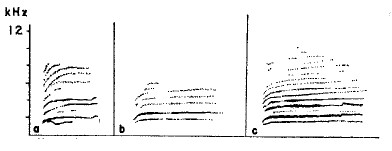
\includegraphics[width=\columnwidth]{figures/sonagraph1}
\caption{Alarm calls of Lawrence's, Lesser, and American Goldfinches
  (\textit{Carduelis lawrencei}, \textit{Carduelis psaltria} and
  \textit{Carduelis tristis}. From Coutlee 1971, Animal Behaviour
  19:559.  This shows the narrowband setting of the Kay Electric
  Company Sonagraph, where frequency resolution is preferred over time
  resolution.}
\label{fig:sonagraph1}
\end{figure}

\begin{figure}[t]
\centering
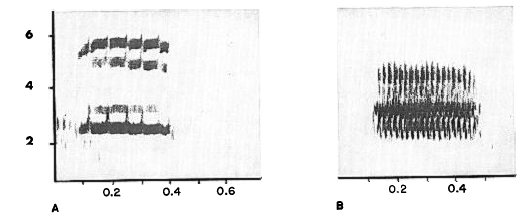
\includegraphics[width=\columnwidth]{figures/sonagraph2}
\caption{The calls of the varied thrush \textit{(Ixoreus
    naevius)}. From Martin 1970, Condor 72:453.  This shows the
  wideband setting of the Kay Electric Company Sonagraph, where time
  resolution is preferred over frequency.}
\label{fig:sonagraph2}
\end{figure}

While originally bioacoustic data was recorded onto wax cylinders, for
most of the 20th century, audio was recorded onto analog magnetic
tapes.  These tapes were capable of storing large amounts of data and
allowed researchers to more easily record the sounds of animals in the
field and the lab.  Analog audio tapes were supplemented by the
introduction of Digital Audio Tapes (DAT) by Sony in 1987.  However,
one limitation of both of these forms of storage is the long time it
takes to fast forward to a particular place on the tape due to the
linear way that the data is stored.  In our system, data is stored
non-linearly, and any part can be accessed in a random access manner
which allows for easier interaction with the data.

\subsection{Orcas - Bioacoustics}
\label{sec:relatedWork:orcasBioacoustics}

There is a considerable, but not immense, literature on the study of
the bioacoustics of \textit{Orcinus orca}, also known as the Killer
Whale.  

One of the earliest work in the analysis of pulsed calls was made by
Watkins \cite{watkins1967harmonic}. Pulsed calls were identified by
Watkins to be pulses of tones, and he provided a detailed analysis of
the spectral qualities of these tones, noting that when studying
pulsed calls, the nature of the pulses has a strong impact on the
spectrogram and gives rise to a banded structure, and that the
distance between the bands gives the repeat rate of the pulses; this
is also known as the Side Band Interval (SBI).  In later work,
especially the catalog of orca vocalizations by Ford
\cite{ford1987catalogue}, the SBI is one of the primary audio features
used in classifying orca calls.  However, in the case of the Orchive,
due to the extreme distance of an orca from the hydrophone this
harmonic structure is often not seen, which limits the use of the SBI
in this work.

Another early study was described by a paper in 1967 by Singleton and
Poulter \cite{singleton1967spectral} in which a detailed spectral
analysis of the call types of captive killer whales was carried out.
This study used a digital approach in which a Fast Fourier Transform
was used to produce a spectrogram of short regions of audio.  This
paper provides a fascinating glimpse into the use of the FFT and DFT
and used the recently developed FFT \cite{cooley1965algorithm} as a
way to dramatically speed up the calculation of spectrograms.  With
the ubiquity of the FFT algorithm, it is interesting to think of a
time when the computational complexity of doing this basic function
was $O(N^2)$ when using the naive DFT, instead of $O(N log(N))$ for
the FFT.  Although a large part of the speedup in solving problems has
been due to the increase of computer performance, theoretical results
such as the FFT which improve the raw algorithm can have dramatic
results on the real world performance of these algorithms.


The structure of the sound producing organs in odontocetes in general
was described in detail by Cranford \cite{cranford1996morphology} who
found that the tissues responsible included a structure that resembled
lips and was made of connective tissue, a cartilaginous blade, a stout
ligament and an array of air sacs made of soft tissues.  This sound
producing organ is capable of producing two sounds at once in a
process known as ``two voice phenomena'', which is also sometimes
called ``biphonation'' by some researchers.  In a recent work by
Madsen \cite{madsen2013nasal} it was found that odontoces use one set
of phonic lips to produce whistles, and another to make clicks, which
means that these sounds are not true biphonation, and are more
correctly two voice phenomena \cite{wilden1998subharmonics}.
Researchers have noted that the sounds that could be produced included
clicks, whistles, and a sound that was the combination of both, a
pulsed call that could contain both a Lower Frequency Component (LFC)
and Upper Frequency Component (UFC).  In later papers
\cite{cranford2000impulse} \cite{cranford2006nasalizations}, they
described this sound producing organ in more detail.  Brown
\cite{brown2008math} did a study of the mathematical implications of
this pulsed biphonation extending the earlier results of Watkins
\cite{watkins1967harmonic}.

A paper in 1982 by Dahlheim and Awbrey
\cite{dahlheim1982classification} provided a classification of the
sounds of captive killer whales.  These whales had been taken from
British Columbia, and a number were identified to be NRKW, which makes it very relevant to this thesis.  In
this paper, they describe 11 different categories of sounds; these are
upscreams, downscreams, creaks, whines, whistles, tones, buzzes,
ricochets, click bursts, chatter and seesaw.  In this paper, they note
that from the different vocalizations, they are able to classify
individuals by oceanarium with high accuracy.  However, it should be
recognized that vocalizations are not the only means that orcas have
of generating sound; for example, there is evidence that they use
tailslaps to disorient herring \cite{simon2005tailslap}, and there are
many instances of a distinct ``crunch'' sound heard on tapes that has
been hypothesized to be the sound of individual salmon being eaten
\cite{helena2012interview}.

An extremely detailed investigation of the vocalizations of the killer
whales off the coast of British Columbia was carried out in a series
of papers by John Ford \cite{ford1982stocks} \cite{ford1983dialects}
that described the group-specific dialects in this population.  In
1987, Dr. Ford published a large catalog of the pulsed calls of the
NRKW \cite{ford1987catalogue}.  In this hugely
important resource, he used a systematic nomenclature to describe a
catalog of approximately 78 different call types with 24 different
subtypes.  The call types were labeled starting with the letter ``N'' for
the NRKW in contrast to call types from the southern
residents, which were prefixed with the letter ``S''.  The call types were
numbered according to the time that they were first encountered,
starting with N1.  The recordings were made into Sonagrams using a Kay
Electric company sonograph, and the Side Band Intervals were measured
with an electronic digitizing tablet on an Apple 2 computer.  This
call catalog remains the primary resource for researchers who wish to
study orca call types, and it has been hugely relevant to the research in
this thesis.

The call types in this call catalog were examined in more detail in a
paper in 1989 by Ford \cite{ford1989acoustic}.  In this paper, the
vocalizations of NRKW are divided into three categories: ``clicks'',
``whistles'' and ``pulsed calls''.  The clicks were short pulses of
sound that were typically made in series, with a variable duration of
between 0.1ms and 25ms and could range in repetition rate from a few
pulses per second to over 300 per second.  These clicks were
identified to be primarily of use in echolocation.  Some orcas do
considerable amounts of echolocation to navigate, locate other group
members and locate prey \cite{barretlennard1996echolocation}.
Whistles were the second type of sound and are a single narrow band
tone with little or no harmonic structure.  He noted that these
whistles were between 1.5kHz and 18kHz and ranged in duration from
50ms to 12 seconds.  These whistles were of widely varying character
with some whistles being stereotyped \cite{riesch2006stability} and
some being in the ultrasonic range \cite{samarra2010killer}
\cite{simonis2012high} \cite{filatova2012ultrasonic}.

The third type of vocalization are pulsed calls, and these are the
primary call types of interest both in the work of Ford and others and
also of this thesis.  They are of a pulsed nature; that is, they have
a central tone that is rapidly pulsed with abrupt and pattern shifts
between pulse rates.  Pulses typically had repetition rates of between
250-2000Hz and a primary energy of between 1 and 6kHz.  He noted three
categories of pulsed calls: discrete, variable and aberrant calls.
Discrete calls had distinctive structural characteristics and were
repetitive, variable calls were modified versions of these discrete
calls, and aberrant calls were clearly based on discrete calls but
were heavily modified.  In this paper, he studied the amount of these
three classes of call types in different behavioural circumstances,
that of foraging, traveling, resting, socializing and beach rubbing,
and found that more variable and aberrant calls occurred during
socializing and beach-rubbing.  He also did a transition state matrix
of the different call types and found clear evidence that certain call
types were more likely to be followed by other call types.  The most
striking of these was the N7/N8 pair of call types, in which an N8
call was always preceded by an N7 call.  This paper is very relevant
to this thesis in that it presents a theoretical structure for
classifying orca call types and for the study of their vocalizations.
Although it describes results from a large amount of data, the number
of recordings in the Orchive is even larger, and testing the
hypotheses stated in this paper with a larger dataset could be
enlightening in the study of orca call types.

Orcas from different parts in the world also have discrete call types that
are diverse, and a study by van Parijs \cite{parijs2004norwegian} on
Norwegian killer whales found that none of the call types recorded matched
with those of a previous call catalog \cite{strager1995call}.  Another
earlier study by Steiner et al. \cite{steiner1979vocalizations} looked
at the vocalizations and feeding behaviour of orcas.  Discrete call
repertoires are thought to be mainly to promote group cohesion and to
coordinate intragroup activities \cite{ford1989acoustic}
\cite{ford1991vocal}.  Dolphin signature whistles function as cohesion
calls when a social group is separated \cite{janik1998context}
\cite{watwood2005signature}.  Resident orcas increase use of family
specific call types after calves are born \cite{weiss2006vocal},
particularly between mothers and their dependent offspring.

A recent study \cite{miller2004matching} conducted with Northern
Resident Killer whales found that there was evidence for call type
matching in vocal exchanges.  Further work by this same group
\cite{miller2006diversity} found that discrete calls are at an
amplitude that far exceeds the intra-group separation of members and
likely function in inter-group communication.  Work by this group
found that individual orcas tend to match call types produced by other
group members \cite{miller2004matching} and this can assist group
cohesion \cite{miller2002mixed} and allow individual recognition
\cite{miller2007caller}.

A study using data from OrcaLab, but before the Orchive was created
\cite{weiss2006vocal}, found that orcas change their call behaviour in
the presence of other groups of whales increasing the number of
matriline-specific, variable and aberrant calls, and decreasing the
number of low arousal calls.  The calls also changed more when a
different subclan was in the area and might play a role in
coordination of inter-group activity.

Janik \cite{janik1999pitfalls} did a study on the classification of
dolphin whistles using humans versus an algorithmic approach and found
a greater probability of humans to identify signature whistles than
algorithmic-based approaches.  This is highly relevant to this thesis
in that it highlights the importance of using external validation in
studying vocalizations, and the serious casual game interface allows
researchers to easily create new experiments for humans to identify
calls.  These results can then be compared with algorithmic based
approaches to validate their performance.  Recent work by Janik and
King et al. \cite{king2013copying} suggests that the use of vocal
copying plays an an important role in the social behaviour of dolphins,
and that dolphins can learn the vocalizations of other dolphins.

In a recent paper by Yurk et al. \cite{yurk2010sequential} they note
that due to vocal difference between clans, acoustic monitoring is a
good way to monitor populations of orcas \cite{barretlennardphd} and
identified 7 different pods of whales.  The life history and
population dynamics of this population have also been studied
\cite{olesiuk1990life}.  There has been considerable research into
their behaviour and vocalizations \cite{thomsen1999orca} and their
whistles \cite{thomsen2001whistles} and their significance
\cite{thomsen2002significance}.  The sequences of whistles in Northern
Resident Killer whales has been studied \cite{riesch2008sequences} and
evidence has been shown of vocal learning in orcas
\cite{deecke2000dialect}.  Orcas have the ability to make two
different tones at once, a pulsed lower frequency component made by
one nasal plug, and a tonal upper frequency component made by the
other.  There has been a study to examine the effects of the sex of
the calling whale on the spectral characteristics \cite{miller07sex}
of the vocalizations.  The variation in the pitch of calls in orcas in
different ecotypes as was shown to have \cite{foote2008variation}
significant variation in call pitch.

The evolution of pulse click use in odontocetes is examined in a paper
by Morisaka and Connor \cite{morisaka07predation} and other work on
pulse clicks for echolocation has been reported
\cite{simon07echolocation}.  A study of the auditory brainstem
response of orcas has been presented \cite{szymanski1999brainstem} and
a related paper \cite{hemil2001mass} looks at how high frequency
hearing in odontocetes is affected by bone mass.  There has also been
a study on how automatic gain control is handled in the odontocete
brain \cite{supin2008forward}, an interesting result that should be
taken into account if one were to design electronic analogs
\cite{lyon1982cochlea} of a odontocete cochlea.

Other studies on orcas have included the effects of organochlorine on
their life history \cite{ylitalo2001organochlorine} and of how
persistent organic pollutants affect chinook salmon
\cite{cullon2009pollutants}, which are one of the main prey items of
NRKW.

There have been other studies of marine mammals with fixed hydrophones
including humpback whales \textit{Megaptera novaeangliae}
\cite{norris1999humpback}, bowhead whales \textit{Balaena mysticetus}
\cite{cummings1985pam}, blue whales \textit{Balaenoptera musculus}
\cite{stafford1998longrange} and killer whales
\cite{morton2002displacement}.  In this study, the remote hydrophone
station was manned by a single observer who had to manually do the
recordings of the different pods.  In this thesis I describe a system
that could be used for the automated detection and recording of orca
calls, thus allowing more sites to be observed and the reduction of
human effort.

However, most of the work in analyzing orca vocalizations has been
painstakingly done by hand, sometimes using audio cassettes and expert
knowledge of orca vocalizations, and sometimes by digitizing
vocalizations into a computer and then analyzing spectrograms.  It
would be of advantage to the field to be able to apply these
algorithms to a large dataset and provide collaborative visualization
tools to explore it.

\subsection{Orcas - Algorithms}
\label{sec:relatedWork:orcasAlgorithms}

For a number of years, computers have been applied to the study of
orca vocalizations.  One very early work is by Singleton and Poulter
\cite{singleton1967spectral} where they use an FFT to make
spectrograms of orca vocalizations.

A work by Deecke \cite{deecke1999quantifying} used neural networks to
determine similarity between orca vocalizations.  In this paper, they
found that neural networks were able to predict similarity between
call types with an accuracy comparable to that of expert human
listeners.  Another algorithm that has been applied to this problem
domain is that of Dynamic Time Warping \cite{deecke2006pitfalls}.
Brown et al. \cite{brown2006classifying} \cite{brown2007dtw}
investigate the use of DTW for calculating similarity between two orca
vocalizations and find that this algorithm performs very well.

The mathematical foundations of the pulsed vocalizations by orcas have
also been studied \cite{brown2008math}.  In this paper, formulas for
their spectra are rigorously derived from the basic formulas of
Fourier analysis.  This paper describes in detail the complex spectra
that are able to be produced by orcas and the biological foundations
that underlie them.

Another mathematical method that has been used to describe orca
vocalizations is the Hilbert-Huang transform, which has been shown
\cite{adam2006hilbert} to have advantages over using traditional
Fourier based methods of calculating spectra for bioacoustic sounds.

One important pitfall in the automated classification of orca
vocalizations is that there exist non-linearities in sound perception
in all animals, including orcas\cite{nummela1999anatomy}.

By definition, orca pulsed calls contain a Low Frequency Component
(LFC) with fundamental frequency between 80 and 2.4kHz; however, it
was found that some also contain a High Frequency Component (HFC) with
fundamental frequency between 2 and 12kHz \cite{hoelzel1986call}.
However, these HFCs are more directional than the LFCs
\cite{miller2002mixed}, and because orcas are seldom pointing directly
at a hydrophone, these are often not clearly seen in OrcaLab
recordings.  Another challenging factor in studying orca vocalizations
is that two or more different orcas can be making calls at one time,
and to determine call identity, these overlapping calls need to be
separated \cite{ford1987catalogue}.

Several studies found considerable individual variability of orca
vocalizations \cite{miller2000orca} \cite{nousek2006social}
\cite{parijs2004norwegian}.  A groundbreaking study by Deecke
\cite{deecke2000dialect} found evidence for cultural transmission
of vocalizations in orca populations.  A real-time system with low
computational requirements for the detection of Orca vocalizations is
described in \cite{luke2010realtime}.

In a paper by Miller and Bain \cite{miller2000variation}, they noted
that discrete calls always have a LFC and often end in a ``terminal
note'', a relatively short feature at the end of a call separated by
the rest of the call by a rapid change in the slope or frequency of
the LFC.  Within a call type, they found that the UFC was highly
stereotyped.  The similarity between call types correlated highly with
how often the matrilinear units (MU) associated with one another,
which was from previous work by Bigg et al. \cite{bigg1990orca}.

Recordings often have large amounts of boat noise in them due to the
large and increasing amount of marine traffic in the Johnstone
Strait and around Hanson Island.  Many OrcaLab recordings are done
remotely using standard sonobuoy transmitters, which makes their quality
similar to telephone calls; thus, algorithms that are designed to
handle noise are useful \cite{wang2000pitch}.  However, these
algorithms often depend on harmonic structure, and for many OrcaLab
recordings, the orcas are distant from the hydrophones, and there is
not much harmonic structure visible on spectrograms.

Deecke describes two different ways to classify vocalizations
\cite{deecke1999quantifying}.  The first he calls statistical and is
obtained by looking at properties and statistics of the pitch track.
He notes that these methods only assess physical properties of the
signal and not how they are perceived.  The other method is
perceptual, and in this method, humans (or animals) listen to the
pitch and classify them.  The advantage of this is that factors that
are missed by a Digital Signal Processing approach might be detected
by the sophisticated auditory systems present in living beings.  One
downside of this approach is observer bias.  Another is that orcas and
dolphins have more inner hair cells in their peripheral auditory
system than humans \cite{au2000hearing}.  This is of direct relevance
to this thesis in that I provide functionality to allow the use of
data from both human observers using a perceptual metaphor as well as
what Deecke calls statistical methods which are called audio features
in this thesis.

A further contribution from Deecke in the same paper
\cite{deecke1999quantifying}, shows results from the Sidewinder
algorithm, which uses autocovariance of FFT with a neural network.
They compare these results to those by humans who had no knowledge of
orca vocalizations and show that the algorithm performed well even
with poor SNR.  The advantages of the Sidewinder algorithm is that it
uses more points that other analyses that just use a few points on the
pitch contour (min, max, etc. \cite{au2000hearing}).  The
disadvantages to its use are that it had problems when noise had a
harmonic component, that it cannot be applied to broadband or pure
tone signals, that it does not take amplitude into consideration, and
that it is computationally expensive compared to other approaches.
The authors suggest that it can be used in combination with other
algorithms.  This paper showed that using a neural net to classify the
output of the Sidewinder algorithm and the perceptual approach using
human volunteers gave similar results.  Unfortunately, preliminary
tests showed that the Sidewinder algorithm is of limited use on the
data from the Orchive because of the often limited harmonic structure
of the recordings.

A very early study by Watkins \cite{watkins1967harmonic} on pulsed
calls noted that the highest energy is not always contained in the
first, second or third harmonics.  This is often seen in the
recordings in the Orchive, and this can cause problems with pitch
estimation algorithms that assume that the fundamental frequency has
the highest energy.

In a paper by Au et al. \cite{au2004echolocation} the echolocation
clicks of orcas were measured and analyzed in detail.  They estimate
that orcas would be able to detect salmon at a distance of 100m even
in the presence of heavy rain noise.  They also mention that boat
noise is of a different character than rain and wind noise, and the
impact of boat noise on echolocation is unknown.  This paper is of
relevance to this thesis in that, in the data in the Orchive, there
are many such recorded echolocation clicks, and a deeper understanding
of these clicks and how orcas adapt their echolocation behaviour in
the presence of noise could be a useful contribution to the
literature.  This theme of the impacts of noise on Orca communication
can also be found in \cite{holt2009speakingup}, where the impacts of
noise on the southern resident killer whale (SRKW) population is
examined.  In this paper they found that when boat noise increased by
1dB, orcas raised their volume of their calls by 1dB.

Janik \cite{janik1999pitfalls} studies the use of three different
algorithmic techniques to compare dolphin whistles.  The first is
based on an algorithm by McCowan \cite{mccowan1995quantitative} that
first normalizes the length of each call and then takes 20 points
along its length as independent variables.  These then used as input
to a Pearson product-moment correlation matrix, which then gives a
similarity measure between pairs of whistles, which was then subjected
to Principal Component Analysis to reduce the number of colinear
variables.  These values were then used as input to a k-means
clustering algorithm.  This paper also used two cross-correlation
based methods, one that used the cross-correlation of two signals using
a method described by Khanna et al. \cite{khanna1997crosscorrelation},
and the other that used the same cross-correlation, but instead took
the absolute difference in frequency every 5ms.

Considerable work has gone into the identification of dolphin
signature whistles in the last two decades \cite{sayigh1990signature}.
A recent paper by Janik et al. \cite{janik2013signature} presents a
new method for identifying dolphin signature whistles called SIGnature
IDentification (SIGID), which uses the observations of human listeners
followed by a type of analysis that looks at the gaps between groups
of vocalizations which known as bout
analysis\cite{slater1982minimising}.  Dolphin vocalizations often are
found in a trend where many vocalizations are made close in time with
large gaps between them, which makes them amenable to study by bout
analysis.  In the Janik experiment \cite{janik2013signature}, they
found that they could reliably detect individual dolphins in
recordings of groups of dolphins with the SIGID technique.  This
research is explained in greater depth of the Ph.D. thesis of King
\cite{king2012imitation} where the use of signature whistles as vocal
labels amongst other topics is examined.  This is of relevance to the
current thesis in that I present an extensible computer system that
would allow researchers to conduct the human study portion of the
SIGID system using citizen scientists.

Other interesting work on dolphin communication is presented in a
recent paper by Janik \cite{janik2013cognitive} in which the
capability of dolphins to refer to objects and other dolphins using
referents and their ability to understand syntactic structure is
reviewed.  This paper is of relevance in that orcas are of the same
taxonomic family as are dolphins and could possibly share some of
their cognitive abilities.

One approach to determining the fundamental frequency of a
vocalization is to manually trace spectrogram by hand using
appropriate software; for example, in Watwood et
al. \cite{watson2004biodiversity} the MATLAB software suite is used to
this end.  A paper by Shapiro et. al
\cite{shapiro2006signature} uses this same approach.  While this
approach is appropriate for small datasets, it is most likely
untenable for the multi-thousand hour datasets explored in this
thesis.

Another approach that has been used is to select peak frequency from
sliding power spectrum followed by manual correction to remove octave
errors \cite{buck1993quantitative} \cite{janik1994signature}.  In
previous work in our lab \cite{ness2008chants}, this approach was also
used by hand with MATLAB, and in our software suite, I have
functionality that allows a user to select a wide variety of
parameters for pitch determination algorithms that brings this same
functionality to a web-based interface.

One of the most useful algorithms for determining the pitch contours
of orca calls is the previously described Sidewinder algorithm, which
uses autocovariance for each spectral slice where the peaks are at
multiples of the spacing of frequency bands
\cite{deecke1999quantifying}.  This algorithm is particularly
appropriate to sounds that are of a pulsed-tone nature.  These sounds
are composed of a pure tone that is pulsed at a specific, and perhaps
varying, rate.  A spectrogram of such tones has many bands
\cite{watkins1967harmonic} around a central frequency, with the most
energy occurring near the frequency of the tone and not in the lower
harmonics as is in the sounds of many instruments.  The sidewinder
algorithm is similar to the spectral autocorrelation method for human
speech tracking \cite{lahat1987autocorrelation}.

A similar algorithm is the Discrete-Logarithmic Pitch Detection
Algorithm DLFT-PDA \cite{wang2000pitch}.  The DLFT makes reliable
estimations of pitch and temporal change of pitch from harmonic
structure by correlating DLFT spectra from adjacent frames to give
reliable estimates fundamental frequency change.  It uses Dynamic
Programming to create a smooth pitch track.  However, two drawbacks of
this algorithm are that it performs poorly with low SNR and cannot
track multiple calls by multiple animals.  It was shown to be a a
versatile pitch tracking algorithm in recent work by Shapiro et
al. \cite{shapiro2009pitch}.

Another approach that takes advantage of the banded structure of
pulsed calls is an FFT based comb filter method with Dynamic Time
Warping  \cite{brown2006classifying}.  In this approach, an upsampled
FFT of a sound is produced, and this FFT is then analyzed with a
series of comb filters with equally spaced frequency bands to isolate
the harmonic structures of different repetition rates. This was
explored in \cite{brown2006classifying} and then in more detail in
\cite{brown2007dtw}.  This approach takes as input a pitch contour as
determined by a pitch determination algorithm and can take multiple
pitch tracks to model sounds in which an LFC is combined with an UFC.
The DTW algorithms they explored included the Ellis, Sakoe-Chiba,
Itakura and Chai-Vercoe.  These vary in the way that the cells are
computed, for example in the Chai-Vercoe method, there is explicit
handling of insertions and deletions in the cost matrix.  These
algorithms can be compared to those used in global-sequence alignment
algorithms.  They found that they could get 90\% agreement with
perceptual data, and represented a severe test of DTW, and in their
experiments used both the LFC and UFC components.  The use of DTW
would be an important avenue to pursue in future work.

Another approach used an Artificial Neural Network (ANN) image of
spectrogram transformed into an image of data points then normalized
and transposed into a vector of points which was the input to the ANN
\cite{gaetz1993neural}.  They looked at distinguishing calls from each
other in one experiment and whales from each other in another, both
experiments gave excellent classification accuracy on a small dataset.
However this method has the disadvantage that it is very sensitive to
noise and may do the classification on the noise rather than on the
signal.

A recent study \cite{adam2006hilbert} discusses the use of the
Hilbert-Huang Transform (HHT) for analyzing the sounds of marine
mammals.  They mention that the FFT is limited to the Heisenberg
uncertainty principle, and that time and frequency resolutions must be
chosen by the investigator and relate that the HHT does not suffer
from this drawback.  They say that FFTs are best suited for analyzing
harmonic signals but not for click sounds, while the HHT is better
suited for this.  They provide results that show the effectiveness of
the HHT over the FFT, especially in the case of clicks where when the
ratio between the maximum of the energy when a click is present to
that when the click is absent is approximately 20:1 with the FFT and
is approximately 100:1 with the HHT.  This HHT algorithm would be
useful to implement and test in the future.

Another approach using FFTs to classify whale calls is described by
Oswald et al. \cite{oswald2003acoustic} who use a multivariate
discriminating function analysis for classifying whale vocalizations.
They examine the use of different upper frequency limits (20, 24, 30
and 40kHz) and different variables for each call, including beginning
and ending frequency, minimum and maximum frequency, duration, number
of inflection points, number of steps and if harmonics were present
from the fundamental frequency of each whistle.  They got fairly poor
classification accuracy (37\% at 24kHz) using a multivariate approach
with cross-validation, but their detailed analysis of using these
different parameters was quite useful.  With a more sophisticated
statistical treatment and a dataset larger than the 484 whistles from
29 recording sessions, it might be possible to obtain higher
classification accuracy.

Another more recent approach by Deecke \cite{deecke2006playback} included the
use of the Adaptive Resonance Theory (ART) neural network, a network
similar to the Self-Organizing Map approach in that it is an
unsupervised approach using a neural-net like foundation; however, in
the ART algorithm, if a new pattern is found that is sufficiently
different from existing patterns, it becomes the reference pattern for
a new category.

Another way to classify audio features is to use the Pearson product
moment correlation which was used in Watwood et
al. \cite{watwood2004whistle} to classify the vocalizations of
bottlenose dolphins.  The main advantage of this technique are that it
takes into account the differences that are lost when whistle loops
are normalized in time, it also ignores absolute frequency and
bandwidth information.  By doing so, it makes loops that have
monotonic changes in frequency appear more similar even if they are
considerably different in absolute frequency.

In this section, a number of different algorithms for extracting audio
features from bioacoustic recordings are presented.  The primary
method that is used is typically based on FFTs, however, there has
been work using other algorithms such as the Hilbert-Huang transform
and the Sideband Interval.  To compare different audio features, DTW
has been used with good results, and the ART model has also shown
promise in categorizing bioacoustic sounds.

\section{Systems for working with large audio corpora}
\label{section:relatedWork:systems}

Large amounts of work have been done using single computers to study
large amounts of audio.  Recent advances in storage capacity have led
to very large 4TB disks, so a considerable amount of audio data can be
stored.  However, at a certain point, with many hundreds of terabytes
of audio, research labs often adopt a file server model, where a
central server or set of servers delivers data to client computers.
This methodology is in use at the Cornell Lab of Ornithology
Bioacoustics Research Program (BRP) \cite{clark2012dcl} where a server
connects to a large array of spinning disks and client computers query
this data using powerful workstations.  These workstations use MATLAB
and other software to listen to audio and interact with advanced
custom interfaces.  This approach is similar to the system described
in this thesis in that users can interact with audio using custom
software in both.  One primary difference is that in the case of the
custom MATLAB, it would be challenging to integrate an external
citizen science interface or indeed have the ability to interact with
a non-privileged custom workstation connect via a dedicated high-speed
network to the data.  One design decision that I modeled on the
Cornell system, and am grateful for, was the ability to let users use
their own software platform for doing complex calculations and then
to have easy ways for them to view their data in the context of the
Orchive.  This is accomplished in our system by having multiple ways
for data to be stored, either on a shared file system like NFS, via a
shared folder service like Dropbox, or on their own computer where
they can watch results being added in real time.

A different methodology of doing audio feature extraction was explored
in the paper ``Distributed audio feature extraction for music''
\cite{bray2005distributed}.  In this paper, the authors use a dataflow
architecture for distributed audio feature extraction on a set of
networked computers.  A dataflow architecture allows users to connect
small processing algorithms in a graph-like network and to then use
this constructed network to transform input data into a desired type
of output data.  A simple example of a \textit{Marsyas} network would take
audio samples from a file on disk, multiply them by a number and
output them to another file on disk, which would have the effect of
increasing the volume (loudness) of the file.  However, most of the
commonly used algorithms in \textit{Marsyas} are complex feature extraction and
machine learning algorithms.  \textit{Marsyas} was an existing software
platform that used this dataflow architecture, and this paper explored
the use of dataflow architectures on networked computers.  One of the
important contributions of this paper was that the optimal vector size
of data to send from one computer to the other was influenced by the
network settings of their Ethernet routers, but in their case a 256
size vector provided the best speed.  Results are also presented to
show that by using a Collection Partitioning Adaptive algorithm the
authors were able to get the best utilization of their cluster.  This
algorithm splits up the files to be processed and adaptively sends
more jobs to the computers that have completed their past jobs
quickest.  The authors also note that it is very simple to port an
existing \textit{Marsyas} network to this distributed framework, and there is
indeed current efforts ongoing to do this in an automated fashion.

One serious drawback of this framework is the large amount of disk and
network traffic that is generated by the producer nodes on these
system, the authors point out that the maximum number of worker
computers that could be served by one dispatcher computer was only
four.  This makes sense because of the large amount of data generated
in many of the intermediate steps in the audio feature extraction
pipeline.  The authors propose a system of hierarchical dispatchers
and workers to solve this problem.

For many interesting tasks in realtime computer generated music and
analysis of music in performance situations this type of system would
be very useful, for example, one dispatcher could communicate with a
number of workers each of run a different type of machine learning
algorithm and where the results are then collated.  However, for the
present task of analyzing huge collections of audio that is already on
disk in a batch fashion, the architecture in distributed \textit{Marsyas}
likely would need further work to be of much use.

In ``Overview of OMEN''\cite{mcennis2006omen}, McEnnis, McKay and
Fujinaga describe their system called OMEN (On-demand Metadata
Extraction Network), a system that shares many commonalities with the
Orchive system described in this thesis.  The main issue their
system aims to overcome is copyright problems that researchers
encounter when they want to legally extract audio features from songs.
In the strictest legal sense, each researcher must purchase their own
version of a song in order to do any kind of audio science on it.
This becomes prohibitive in the age of online databases with millions
of songs in them.  In the OMEN system, a coalition of libraries
creates a network of systems that host the raw audio data of the song
but only send back to the researchers the specific audio features that
they are interested in.  Another interesting aspect of this system is
that they propose to use the unused computing cycles of library
browsing computers to be a grid computing resource for doing their
audio feature extraction.

One big difference is that their system is primarily based on
Java \footnote{\url{http://www.oracle.com/technetwork/java/index.html}},
where the system described in this thesis is primarily based on
Python, C++ \footnote{\url{http://www.open-std.org/jtc1/sc22/wg21/}}
and Javascript \footnote{\url{http://www.ecmascript.org/}}.  In many
ways, the Java ecosystem is enticing for building server applications,
and several times in this project I considered doing feature
extraction in jMIR, the Java Music Information Retrieval library that
the OMEN system happens to use.  I decided not to because of greater
performance of \textit{Marsyas} and that it includes more audio feature
extractors.  Another important reason is that \textit{Marsyas} has a mode where
features can be extracted and predicted in one executable which is
very helpful when working on huge datasets such as those in the
Orchive.

\section{Intelligence Augmentation}
\label{section:relatedWork:intelligenceAugmentation}

With the analog tapes from OrcaLab now digitized, it is possible for
researchers to search for, listen to, view and make annotations on all
these \totalNumberOfOrchiveRecordings recordings.  These annotations
can be shared with other researchers or used as input to audio feature
extraction and machine learning algorithms to find specific
vocalizations in large bioacoustic collections.  This type of work
falls under the rubric of Computer Supported Collaborative Work
\cite{bannon1991cscw} (CSCW), a field which studies multiple
individuals working together with computer systems.

In this particular case, there are a number of different communities
who could be interested in this archive, these include developers of
bioacoustic algorithms who include members of the machine learning
community \cite{clark2012dcl} and researchers in Music Information
Retrieval.  Others who might show interest are OrcaLab and its
collaborators, whale biologists, linguists and the part of the general
public who enjoy listening to whales and might like to help the
scientists who are working on this project.

Our system uses two types of web based interfaces.  The first are
tools aimed at expert users, and the second are simpler interfaces
designed for crowdsourcing the annotation. There are a number of tools
that experts use to segment and analyze audio and specifically
bioacoustic data.  One of the most popular is Raven
\footnote{\url{http://www.birds.cornell.edu/raven}}, a toolkit
developed at the Cornell Lab of Ornithology.  Our expert-based tools
have many similarities to Raven such as the ability to view waveforms
and spectrograms at multiple levels of detail. In addition, the system
described in this thesis tightly integrates the visualization and
viewing of data from machine learning classifiers.

Another tool is the Sonic Visualizer \cite{cannam2010sonic}, which
supports a wide variety of waveform and spectral audio
representations. The popular audio program Audacity has been extended
to allow for the annotation of audio data \cite{li2006auacity}.  The
biggest difference of our system compared to these systems is that our
software is all web-based, so users do not have to install a separate
program and can more easily view long audio files and analyze data
across multiple recordings by utilizing compute cluster and cloud
resources.

The goal of early research in Artificial Intelligence (AI) was to
build independently intelligent agents that could perform cognitive
tasks.  There were a number of approaches to build such systems.  Some
researchers, such as John McCarthy, chose to build symbolic
manipulation systems where knowledge was represented by formal logic
\cite{mccarthy1968some} Others, such as efforts by Marvin Minsky
\cite{minsky1961steps}, instead attempted to combine several ad-hoc
solutions to create an independent agent.  Most of these systems
failed to take into account that in the real world, intelligent
agents, such as people, are embodied, that is they have a physical
form, and this physical body interacts both with other agents in
social interactions as well as with its environment.

In the 1980's instead of Artificial Intelligence, researchers began to
investigate Intelligence Augmentation \cite{fischer1992beyond}, where
instead of trying to build intelligent systems that were designed to
replace humans, researchers started building systems that would help
people to solve problems, combining the best of human and artificial
problem solving strategies.  These agents were designed to assist
humans and inherently carried within them the idea that intelligence
was embodied and interacts with people and other artificial agents
through social interactions.

An interesting study was carried out by Sumner
\cite{sumner1997cognitive} and investigated embedding agents that
functioned as critics into a design environment.  In a critiquing
approach, an artificial system communicates in a dialog with a human,
suggesting changes to places where there are problems with the design.
The system described in this paper is that of voice menus for a
phone-based interface.  The system is designed by a person or team,
and the system critiques the design in places where the designer has
violated previously determined rule-based constraints.  This work was
extended in a subsequent article \cite{fischer98embedding} where a
system to help designers create kitchens was described.  One
interesting result from these studies was that designers reacted
negatively to being critiqued and began to anticipate the response of
the system and took steps to avoid being critiqued.  This highlights
the importance of making sure the system that is built makes the users
feel that they are empowered and are being supported by the system.

In a debate entitle ``Direct manipulation vs. interface agents''
\cite{schneiderman1997direct}, Ben Schneiderman and Pattie Maes debate
the relative advantages of direct manipulation and software agents.
Direct manipulation is described to be user interface techniques where
large amounts of data are presented to the user on the screen at one
time.  Through a user interface with fast feedback (\textless100ms),
the user navigates through the data.  Software agents, on the other
hand, are described to be long-lived software systems that learn user
preferences and adapt to users, presenting them with data that the
system estimates will be useful to the user.  In this paper, these two
approaches are discussed and contrasted.  It is interesting to note
that by the end of the debate both sides acknowledge benefits to the
other's position, and indeed, as I have seen in the decade since this
debate, systems are being designed that support both direct
manipulation and software agents.  In the Orchive, I am attempting
to design a system that supports both of these paradigms, allowing the
user to directly manipulate large quantities of data, and also provide
software agents that can mediate interactions between users, other
users, annotations from other software agents and the data.

In the paper ``Distributed intelligence: extending the power of the
unaided, individual human mind'', \cite{fischer2006distributed}
Fischer provides an excellent overview of the field of distributed
intelligence, relating it back to work in distributed cognition by
Hollan et. al \cite{hollan2000distributed} as well as tying in other
concepts, such as those of Intelligence Augmentation, advanced
visualization interfaces that exploit the power of the human visual
system making user specific systems, and exploring computing off the
desktop, which includes both large scale and small scale displays.
This paper also explores the difference between ``Tools for
Learning'', which have the goal of educating the user so that they
will be independent of the system and ``Tools for Living'' that help
people do things they could not do themselves.  In the Orchive, I am
developing tools to support both these paradigms.  First, to help
users learn the call types used by the orcas, and second, to help more
advanced users interact with the data, allowing them to ask and answer
research questions.

In the paper ``Collaborative, programmable intelligent agents''
\cite{nardi1998collaborative}, a system that extracts semantic data
from documents using intelligent agents is described.  This paper
talks about the difficulty of creating systems that approximate real
intelligence and instead proposes that I should investigate what
tasks computers are good for, what tasks people are good for, and how
they can best complement each other.  Their goal is to create a system
that works like a reference librarian, taking imprecise requests from
clients and returning relevant results.  They then present a system
called ``Apple Data Detectors'', which uses a collaborative system to
work with the user to fulfill their requests.  This is related to this
thesis in that it reminds us to have humans do what they do best, and
computers to do what they do best.

The field of Distributed Cognition studies the social and
environmental aspects of cognition and realizes that thinking is not
just something that happens in isolated minds but can also take place
in the interactions between minds and their environment.  It was first
formulated into a discrete discipline by Edwin Hutchins, which is
described extensively in his book ``Cognition in the Wild''
\cite{hutchins1996cognition} after his research into the native people
of Papua New Guinea and their system of public litigation
\cite{hutchins1980culture}.  In a classic paper by Hollan, Hutchins
and Kirsh \cite{hollan2000distributed} distributed cognition in
different environments is described.  One of these is on the bridge of
a ship, a location where multiple persons have to work together to
accomplish many simultaneous and shared goals.  In this situation,
people work together, sharing information via intentional and
consequential communication and also offload cognitive tasks to their
environment by the use of maps, displays and other physical objects.
This type of offloading of information to the environment is seen in
the large amount of data objects that OrcaLab produce, from analog
tape and DAT recordings, to lab book pages, incidence reports, single
subpod recordings, maps, photos and videos.  These different
recordings reveal different facets of the life of the orcas, and in
the Orchive interface, I have attempted to include as many of these
as possible.

The practice of Cognitive Ethnography \cite{hollan2000distributed} is
often used to study distributed cognition.  It studies the cognitive
processes that underlie the work that occurs in an environment and
takes into account the effect of the social context of the
participants as well as the way the physical world affects the
process.  Ethnography is a methodology in which researchers study a
system by making direct observations in as natural a setting as
possible \cite{mcgrath1995methodology}.  An ethnographic study of the
different communities involved in the Orchive would be an excellent
long term goal in future work.

In the book ``Distributed cognitions: Psychological and educational
considerations'' \cite{salomon1997distributed}, a number of authors
investigate distributed cognition and give examples of this in a
number of fields, including daily life and education.  One central
theme of this book is that people think in conjunction or partnership
with others and use tools to help them think.  They also note that it
has been observed that the performance of people in teams supported by
computational tools is often superior to people working alone.  They
then investigate how distributed cognition can be harnessed in the
field of education, with the goal of helping students to learn more
effectively.

There has been a long and fruitful history of the application of
distributed cognition in the sciences.  If one adopts a loose
definition of distributed cognition as thought processes that happen
not just in one individual brain but are instead distributed through
a community and are mediated by artifacts, the whole history of
science itself, even back as far as Aristotle, has been an example of
distributed cognition.  In the words of Isaac Newton:

\begin{quote}
 ``If I have seen further, it is by standing on the shoulder of
  giants''.
\end{quote}

However, recent advances in the understanding of the concept of
distributed cognition from researchers in the social sciences,
combined with advances in computer and communication technology could
dramatically increase the speed, facility and ease of communication
between scientists.  These increases could potentially be
revolutionary changes in certain very difficult problem domains.  In
such domains, the problem itself is too big to be solved by one single
researcher and must instead be solved by teams of researchers with the
aid of artifacts that aid cognition.

There are many different such problem domains that require
collaborations between large numbers of users and one is the study of
the vocalizations of whales.

\section{Citizen Science}
\label{section:relatedWork:citizenScience}

Citizen science is a process by which members of the public are
involved in a collaboration with professional scientists to collect
and analyze data.  Although its coinage as a term is rather recent, it
has a well-established history, with one of the earliest examples
being that of Linnaeus who in his Systema Naturae
\cite{linnaeus1758systema} in 1758 asked volunteers from the public to
send him botanical samples from around the world for the development
of his taxonomical system.  Other examples include the establishment
of a system of amateur weather observatories across the US in the
early 1800s by Thomas Jefferson \cite{fiebrich2009history} and the
Christmas Bird Count \cite{lebaron2009bird} of the Audubon society and
Cornell Lab of Ornithology.

However, in recent years the use of networked computers has
dramatically accelerated the ability for scientists and the public to
collaborate on large scale projects.  The term crowdsourcing refers to
a new type of collaboration where non-specialists help expert
scientists \cite{howe08crowdsourcing} and has been used to great
advantage \cite{surowiecki05crowdsourcing} in a number
\cite{bradham08crowdsourcing} of research programs
\cite{travis08crowdsourcing}.  One of the most successful examples is
Galaxy Zoo \cite{anze08galaxyzoo}.  In ``Game-powered Machine
Learning'' \cite{barrington2012game}, Barrington, Turnbull and
Lanckiet describe a system that combines Games With A Purpose (GWAP)
with machine learning in a framework that they call ``Active Machine
Learning''.  In the paragraphs below, I examine these contributions
in greater detail.  Our system uses a GWAP metaphor for the citizen
science part of the game.  It currently has only a few game-like
elements, however results will be demonstrated that show that a
certain subset of users find even this simple game quite engaging.

In the case of the Galaxy Zoo\cite{anze08galaxyzoo}, A group of
astronomers had collected images of many thousands of galaxies and
wanted to characterize them by the chiral handedness of their spiral
structure, that is, were they spinning clockwise or counterclockwise?
It was assumed that there would be an even distribution of these the
two chiral hands, left and right, and any deviations from this would
be an important and surprising result.  Even the most advanced current
computer algorithms are not able to categorize galaxies based on their
handedness, but humans can do this classification easily.  In this
paper, the authors describe their system and results and present
results that indicate that there is a hint of positive correlation of
the distribution of left or right handed rotation for galaxies nearer
than 0.5 Megaparsecs.

Another research program that benefited from crowdsourcing was the
Stardust@home project \cite{mendez06stardust}.  Stardust
\cite{atkins97stardust} was a NASA space mission that flew a
spacecraft through the tail of comet Wild 2, collected dust from the
comet and from interstellar matter using an aerogel and then returned
the satellite to earth.  Comet dust was collected on one side of the
aerogel, and the other side of the aerogel was exposed to interstellar
matter during the entire mission.  The analysis of the particles from
the comet were straightforward due to the high number of particles,
but the analysis of interstellar grains was much more difficult due to
the small size and number of particles.  The Stardust@home project
allowed users from around the world to signup on a website and
interactively view and annotate microscopic images of the aerogel.
There was overwhelming participation by the public, and they were able
to generate results that were useful to the scientists on the project
\cite{atkins97stardust}.  The system described in this thesis is
similar to this project in that they both have a web based interface
for classification.  The Stardust program was one of the inspirations
behind adding a citizen science part to this thesis.

There have been a number of articles that investigate the benefits of
crowdsourcing.  Hong \cite{hong04crowdsourcing} presents results that
show that a group of problem solvers with a diverse background can
outperform smaller groups of experts.  This is of interest in the
current work because there are only a very small number of orca
vocalization experts in the world, but there is a large number of
people who are interested in listening to orca calls as is evidenced
by the traffic on the OrcaLive \footnote{\url{http://orcalive.net}}
forums.

A recent article \cite{kittur08crowdsourcing} describes crowdsourcing
with the Amazon Mechanical Turk system, a web based system where
people can sign up to work on small tasks in return for micropayments.
The advantage with using the Mechanical Turk system is that because
people are paid for their work and have to pass a scientist-defined
test the results obtained might be of higher quality.  The drawback to
this system is that the workers must be paid.  Most scientific
projects have limited budgets, and therefore this type of solution is
often not practical.

The first GWAP was the ESP game \cite{vonahn2004labelling} in which
two users on computers connected to the internet try to guess words
that describe an image.  If both users guess the same word, this word
is then added to the tags to that image and is also added to a list of
forbidden words which forces people to choose new words to describe an
image.  This game has proven immensely popular, with many millions of
tags added to images.  Another such game is Tag-A-Tune
\cite{law2009input}, an input agreement game that has people add tags
to music clips.  These games, and others like them, exploit the
powerful reward system of the human limbic system and are an excellent
way to hold the attention of large numbers of users and generate high
quality data.  The challenge with games-with-a-purpose is to develop a
captivating game experience, but with time and skill, they perhaps
hold the largest potential in terms of sheer size of population for
performing crowdsourcing.

Although many of these projects concentrate on recruiting large
numbers of participants, even small numbers of human volunteers can be
of great use when analyzing bioacoustic data.  Of particular relevance
to this thesis is work done by researchers in cetacean bioacoustics
\cite{ford1991vocal} \cite{yurk2010sequential} \cite{yurkphd}
\cite{king2012imitation} where human volunteers were used to classify
orca and dolphin vocalizations into distinct categories.  These
researchers used different kinds of technology to do this, primarily
not with a computer, but in recent work by Yurk \cite{yurk2010sequential}
\cite{yurkphd} a web-based interface was developed to allow volunteers
to help classify vocalizations.  The results by the human volunteers
were used to help evaluate the performance of machine learning
algorithms.  This has direct relevance to the current work in that in
this thesis I describe a system that extends this work by providing
an integrated system where researchers can upload, annotate and create
new sets of classification tasks for humans to perform.  The system
that I have implemented also adds game-like elements to hopefully
provide greater engagement of the public along with a concomitant
increase in the amount of data collected.

In ``Game-powered Machine Learning'' \cite{barrington2012game},
Barrington, Turnbull and Lanckiet describe a system that combines
Games With A Purpose (GWAP) with machine learning in a framework that
they call ``Active Machine Learning''.  In this framework, the user is
presented with a set of plausible answers by a machine learning
system, these plausible answers are chosen to be as close to the
actual answer as possible, which helps the system train itself on
difficult data most effectively, and also makes the game more fun and
challenging to play since the answers are so close to each other.
This kind of system directly inspired the work I describe earlier
with GWAP and how I am developing a system to let users help us to
classify orca call types.  Work is underway but unfinished in using active
learning to help to make this game fun and challenging.  Experiments
shown in Chapter \ref{chap:evaluation} show that some users find this
game very engaging.  The results also show that the accuracy is high
for many difficult audio classification tasks including distinguishing
call types between different matrilines.

\section{Summary}
\label{section:relatedWork:summary}

In this chapter, I provided a brief literature survey of a few areas
related to large bioacoustic archives.  Each of these topics is of
direct relevance to this thesis and the system that was built for it.

In section \ref{section:relatedWork:bioacoustics}, a literature survey
is presented included the history of bioacoustics and some of the
early machines used to study it.  Bioacoustics is truly an ancient
field, and many people now and through history have used sound to find
and track animals.  In comparatively recent times, electronic
instruments have helped to add a quantitative measure for the sounds.
It is very useful to closely read these early papers and patents, the
systems they developed using analog technology mirror our current
digital technology, and I can and do draw design inspiration from
them.

A fairly detailed literature search of papers relating to the
bioacoustics of orcas is then presented in subsection
\ref{sec:relatedWork:orcasBioacoustics}.  There is quite a large
volume of work on orca vocalizations.  However, I have attempted to do
a very thorough review of the literature relating to the vocalizations
of the NRKW population.  Thanks to people like Michael Biggs, John
Ford and Paul Spong amongst many others, I know an incredible amount
about this population.  There is quite a large literature on this
population, with work done over a long time period.  This is directly
relevant to our thesis in that the work on making call catalogs and
decoding orca vocalization forms the basis for call classification in
this thesis.

This is followed by another subsection
\ref{sec:relatedWork:orcasAlgorithms} devoted just to the algorithms
for studying orca vocalizations.  There is a considerable literature
on this, but I think I have found all the papers in the literature on
this topic, and have expanded into the vocalizations of dolphins.  In
the system I describe in this thesis, I support a large number of the
algorithms discussed, and can easily add new algorithms.  Several of
these, including the Sidewinder algorithm are very interesting and
would be excellent candidates for audio features to extract.

A section on studying the different types of systems that have been
developed for working with large audio corpora is in section
\ref{section:relatedWork:systems}.  There are some very interesting
systems being developed, like the one at Cornell University with
multiple powerful client workstation computers connected to large
amounts of spinning disk and processing data with MATLAB.  I have
modeled several aspects of the system on these other systems for
dealing with large audio datasets.

A section \ref{section:relatedWork:intelligenceAugmentation} on
Intelligence Augmentation highlights the approach I am taking when
building the system used to produce the results in this thesis.  We
are building a system that uses computers to help annotate large audio
collections by computer scientists and obtain help from biologists who
are experts in the vocalizations of the organism under study.  This
system takes the labeled data from the biologists and lets data
scientists choose different audio features and machine learning
algorithms and interactively view their results in a web-based
interface.  Related to this is Section
\ref{section:relatedWork:citizenScience} which is about Citizen
Science, and how by attracting members of the public to a science
project, considerable work can be accomplished.  This is of direct
relevance to the thesis in that I build and test a system that allows
for citizen scientists to help annotate large bioacoustic archives.

